\documentclass{standalone}
\usepackage{tikz}
\usetikzlibrary{patterns, positioning}
\usepackage[sfdefault]{ClearSans} %% option 'sfdefault' activates Clear Sans as the default text font
\usepackage[T1]{fontenc}

\begin{document}
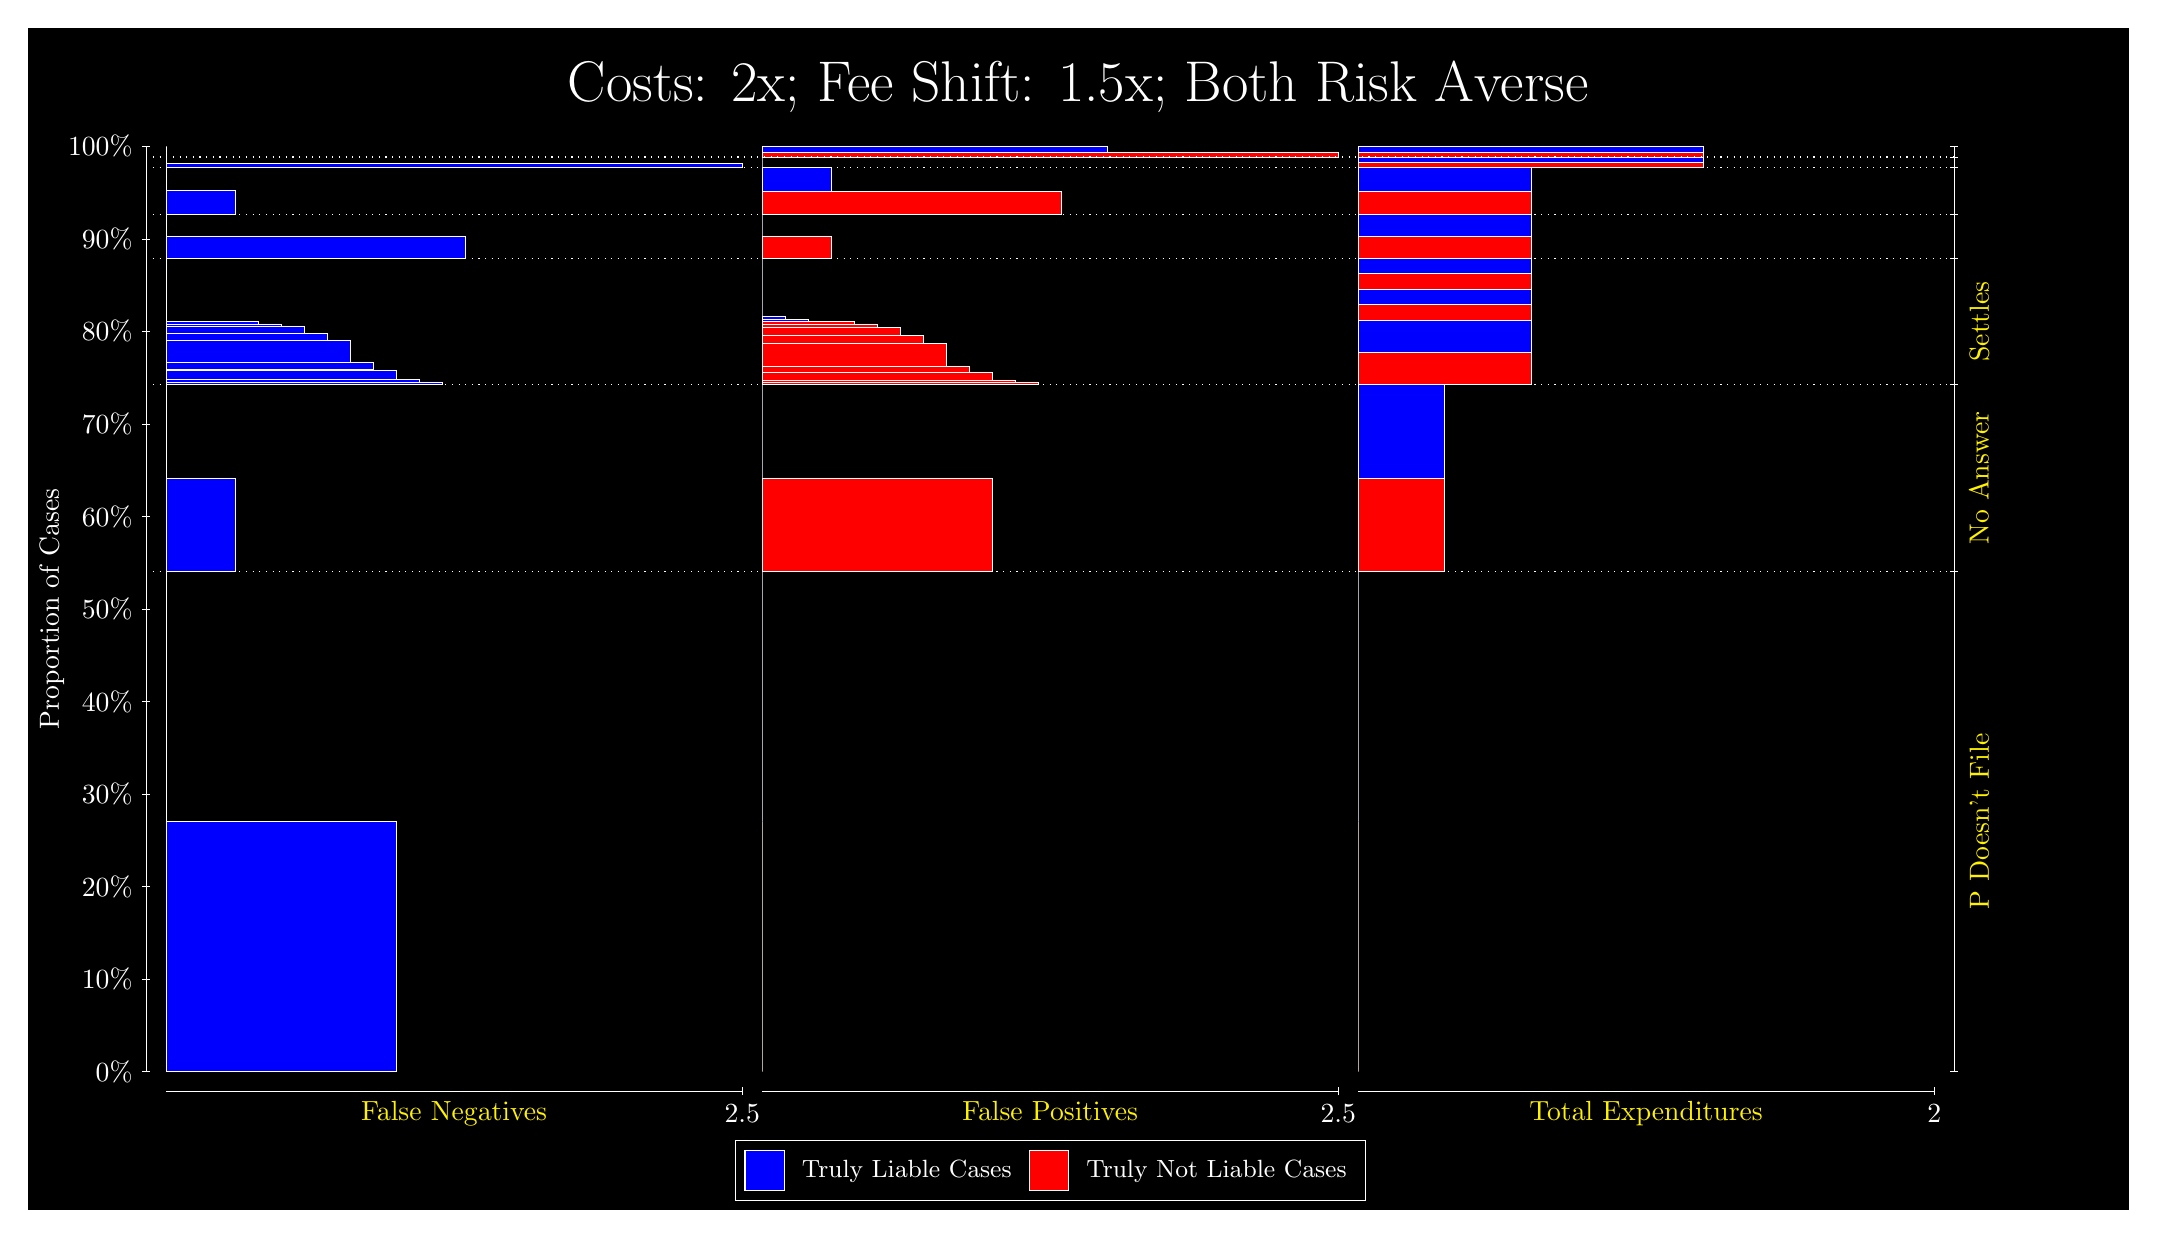
\begin{tikzpicture}
\draw[fill=black] (0,0) rectangle (26.667,15);
\draw[text=white] (0,13.5) rectangle (26.667,15) node[midway] {\huge Costs: 2x; Fee Shift: 1.5x; Both Risk Averse};
\draw[white, very thin] (1.5,1.75) -- (1.5,13.5);
\node[rotate=90, text=white, anchor=center] at (0.3, 7.625) {Proportion of Cases};
\draw[white, very thin] (1.45,1.75) -- (1.55,1.75);
\node[text=white, anchor=east] at (1.45, 1.75) {0\%};
\draw[white, very thin] (1.45,2.925) -- (1.55,2.925);
\node[text=white, anchor=east] at (1.45, 2.925) {10\%};
\draw[white, very thin] (1.45,4.1) -- (1.55,4.1);
\node[text=white, anchor=east] at (1.45, 4.1) {20\%};
\draw[white, very thin] (1.45,5.275) -- (1.55,5.275);
\node[text=white, anchor=east] at (1.45, 5.275) {30\%};
\draw[white, very thin] (1.45,6.45) -- (1.55,6.45);
\node[text=white, anchor=east] at (1.45, 6.45) {40\%};
\draw[white, very thin] (1.45,7.625) -- (1.55,7.625);
\node[text=white, anchor=east] at (1.45, 7.625) {50\%};
\draw[white, very thin] (1.45,8.8) -- (1.55,8.8);
\node[text=white, anchor=east] at (1.45, 8.8) {60\%};
\draw[white, very thin] (1.45,9.975) -- (1.55,9.975);
\node[text=white, anchor=east] at (1.45, 9.975) {70\%};
\draw[white, very thin] (1.45,11.15) -- (1.55,11.15);
\node[text=white, anchor=east] at (1.45, 11.15) {80\%};
\draw[white, very thin] (1.45,12.325) -- (1.55,12.325);
\node[text=white, anchor=east] at (1.45, 12.325) {90\%};
\draw[white, very thin] (1.45,13.5) -- (1.55,13.5);
\node[text=white, anchor=east] at (1.45, 13.5) {100\%};

\draw[white, very thin] (24.457,1.75) -- (24.457,13.5);
\draw[white, very thin] (24.407,1.75) -- (24.507,1.75);
\node[anchor=west] at (24.407, 1.75) {};
\draw[white, very thin] (24.407,8.1001) -- (24.507,8.1001);
\node[anchor=west] at (24.407, 8.1001) {};
\draw[white, very thin] (24.407,10.473) -- (24.507,10.473);
\node[anchor=west] at (24.407, 10.473) {};
\draw[white, very thin] (24.407,12.078) -- (24.507,12.078);
\node[anchor=west] at (24.407, 12.078) {};
\draw[white, very thin] (24.407,12.634) -- (24.507,12.634);
\node[anchor=west] at (24.407, 12.634) {};
\draw[white, very thin] (24.407,13.229) -- (24.507,13.229);
\node[anchor=west] at (24.407, 13.229) {};
\draw[white, very thin] (24.407,13.365) -- (24.507,13.365);
\node[anchor=west] at (24.407, 13.365) {};
\draw[white, very thin] (24.407,13.5) -- (24.507,13.5);
\node[anchor=west] at (24.407, 13.5) {};

\draw[white, very thin, fill=blue] (1.75,1.75) rectangle (4.6775,4.9251);
\draw[white, very thin, fill=red] (1.75,4.9251) rectangle (1.75,8.1001);
\draw[white, very thin, fill=blue] (1.75,8.1001) rectangle (2.6283,9.2866);
\draw[white, very thin, fill=red] (1.75,9.2866) rectangle (1.75,10.473);
\draw[white, very thin, fill=blue] (1.75,10.473) rectangle (5.2631,10.508);
\draw[white, very thin, fill=blue] (1.75,10.508) rectangle (4.9703,10.541);
\draw[white, very thin, fill=blue] (1.75,10.541) rectangle (4.6775,10.652);
\draw[white, very thin, fill=blue] (1.75,10.652) rectangle (4.3848,10.672);
\draw[white, very thin, fill=blue] (1.75,10.672) rectangle (4.3848,10.752);
\draw[white, very thin, fill=blue] (1.75,10.752) rectangle (4.092,11.04);
\draw[white, very thin, fill=blue] (1.75,11.04) rectangle (3.7993,11.123);
\draw[white, very thin, fill=blue] (1.75,11.123) rectangle (3.5065,11.215);
\draw[white, very thin, fill=blue] (1.75,11.215) rectangle (3.2138,11.244);
\draw[white, very thin, fill=blue] (1.75,11.244) rectangle (2.921,11.276);
\draw[white, very thin, fill=red] (1.75,11.276) rectangle (1.75,12.078);
\draw[white, very thin, fill=blue] (1.75,12.078) rectangle (5.5558,12.352);
\draw[white, very thin, fill=red] (1.75,12.352) rectangle (1.75,12.634);
\draw[white, very thin, fill=blue] (1.75,12.634) rectangle (2.6283,12.936);
\draw[white, very thin, fill=red] (1.75,12.936) rectangle (1.75,13.229);
\draw[white, very thin, fill=blue] (1.75,13.229) rectangle (9.0689,13.291);
\draw[white, very thin, fill=red] (1.75,13.291) rectangle (1.75,13.365);
\draw[white, very thin, fill=red] (1.75,13.365) rectangle (1.75,13.427);
\draw[white, very thin, fill=blue] (1.75,13.427) rectangle (1.75,13.5);
\draw[white, very thin, fill=red] (9.3189,1.75) rectangle (9.3189,4.9251);
\draw[white, very thin, fill=blue] (9.3189,4.9251) rectangle (9.3189,8.1001);
\draw[white, very thin, fill=red] (9.3189,8.1001) rectangle (12.246,9.2866);
\draw[white, very thin, fill=blue] (9.3189,9.2866) rectangle (9.3189,10.473);
\draw[white, very thin, fill=red] (9.3189,10.473) rectangle (12.832,10.505);
\draw[white, very thin, fill=red] (9.3189,10.505) rectangle (12.539,10.533);
\draw[white, very thin, fill=red] (9.3189,10.533) rectangle (12.246,10.626);
\draw[white, very thin, fill=red] (9.3189,10.626) rectangle (11.954,10.711);
\draw[white, very thin, fill=red] (9.3189,10.711) rectangle (11.661,10.997);
\draw[white, very thin, fill=red] (9.3189,10.997) rectangle (11.368,11.095);
\draw[white, very thin, fill=red] (9.3189,11.095) rectangle (11.075,11.207);
\draw[white, very thin, fill=red] (9.3189,11.207) rectangle (10.783,11.24);
\draw[white, very thin, fill=red] (9.3189,11.24) rectangle (10.49,11.275);
\draw[white, very thin, fill=blue] (9.3189,11.275) rectangle (9.9044,11.307);
\draw[white, very thin, fill=blue] (9.3189,11.307) rectangle (9.6116,11.336);
\draw[white, very thin, fill=blue] (9.3189,11.336) rectangle (9.3189,12.078);
\draw[white, very thin, fill=red] (9.3189,12.078) rectangle (10.197,12.36);
\draw[white, very thin, fill=blue] (9.3189,12.36) rectangle (9.3189,12.634);
\draw[white, very thin, fill=red] (9.3189,12.634) rectangle (13.125,12.928);
\draw[white, very thin, fill=blue] (9.3189,12.928) rectangle (10.197,13.229);
\draw[white, very thin, fill=red] (9.3189,13.229) rectangle (9.3189,13.303);
\draw[white, very thin, fill=blue] (9.3189,13.303) rectangle (9.3189,13.365);
\draw[white, very thin, fill=red] (9.3189,13.365) rectangle (16.638,13.427);
\draw[white, very thin, fill=blue] (9.3189,13.427) rectangle (13.71,13.5);
\draw[white, very thin, fill=red] (16.888,1.75) rectangle (16.888,4.9251);
\draw[white, very thin, fill=blue] (16.888,4.9251) rectangle (16.888,8.1001);
\draw[white, very thin, fill=red] (16.888,8.1001) rectangle (17.986,9.2866);
\draw[white, very thin, fill=blue] (16.888,9.2866) rectangle (17.986,10.473);
\draw[white, very thin, fill=red] (16.888,10.473) rectangle (19.083,10.88);
\draw[white, very thin, fill=blue] (16.888,10.88) rectangle (19.083,11.289);
\draw[white, very thin, fill=red] (16.888,11.289) rectangle (19.083,11.489);
\draw[white, very thin, fill=blue] (16.888,11.489) rectangle (19.083,11.688);
\draw[white, very thin, fill=red] (16.888,11.688) rectangle (19.083,11.883);
\draw[white, very thin, fill=blue] (16.888,11.883) rectangle (19.083,12.078);
\draw[white, very thin, fill=red] (16.888,12.078) rectangle (19.083,12.36);
\draw[white, very thin, fill=blue] (16.888,12.36) rectangle (19.083,12.634);
\draw[white, very thin, fill=red] (16.888,12.634) rectangle (19.083,12.928);
\draw[white, very thin, fill=blue] (16.888,12.928) rectangle (19.083,13.229);
\draw[white, very thin, fill=red] (16.888,13.229) rectangle (21.279,13.303);
\draw[white, very thin, fill=blue] (16.888,13.303) rectangle (21.279,13.365);
\draw[white, very thin, fill=red] (16.888,13.365) rectangle (21.279,13.427);
\draw[white, very thin, fill=blue] (16.888,13.427) rectangle (21.279,13.5);
\draw[white, dotted] (1.5,8.1001) -- (24.457,8.1001);
\draw[white, dotted] (1.5,10.473) -- (24.457,10.473);
\draw[white, dotted] (1.5,12.078) -- (24.457,12.078);
\draw[white, dotted] (1.5,12.634) -- (24.457,12.634);
\draw[white, dotted] (1.5,13.229) -- (24.457,13.229);
\draw[white, dotted] (1.5,13.365) -- (24.457,13.365);
\draw[white, very thin] (1.75,1.5) -- (9.0689,1.5);
\node[text=yellow, anchor=north] at (5.4094, 1.5) {False Negatives};
\draw[white, very thin] (9.0689,1.45) -- (9.0689,1.55);
\node[text=white, anchor=north] at (9.0689, 1.45) {2.5};

\draw[white, very thin] (9.3189,1.5) -- (16.638,1.5);
\node[text=yellow, anchor=north] at (12.978, 1.5) {False Positives};
\draw[white, very thin] (16.638,1.45) -- (16.638,1.55);
\node[text=white, anchor=north] at (16.638, 1.45) {2.5};

\draw[white, very thin] (16.888,1.5) -- (24.207,1.5);
\node[text=yellow, anchor=north] at (20.547, 1.5) {Total Expenditures};
\draw[white, very thin] (24.207,1.45) -- (24.207,1.55);
\node[text=white, anchor=north] at (24.207, 1.45) {2};

\node[text=yellow, centered, rotate=90] at (24.777, 4.9251) {P Doesn't File};
\node[text=yellow, centered, rotate=90] at (24.777, 9.2866) {No Answer};
\node[text=yellow, centered, rotate=90] at (24.777, 11.276) {Settles};





\draw (12.978300999999998,1.5) node[draw=none] (baseCoordinate) {};
\begin{scope}[align=center]
        \matrix[scale=0.5, draw=white, below=0.5cm of baseCoordinate, nodes={draw}, column sep=0.1cm]{
            \node[rectangle, draw, minimum width=0.5cm, minimum height=0.5cm, fill=blue] {}; &
            \node[draw=none, font=\small, text=white] (B) {Truly Liable Cases}; &
            \node[rectangle, draw, minimum width=0.5cm, minimum height=0.5cm, fill=red] {}; &
            \node[draw=none, font=\small, text=white] (B) {Truly Not Liable Cases}; \\
            };
\end{scope}

\end{tikzpicture}
\end{document}